\section{Overview}
To ease the maintenance and ensure scalability, we have structured the project in an architecture which supports scalability.
The architecture consists of four macro components and a database, as can be seen in \cref{fig:architecture}. The macro components are: Shared, Location Service, Model Agent, and Web Service.\alexander{Maybe change the component name of `Model Updater' so it does not conflict with the layer name? \alexander{Changed name of component to `Model Agent'.}}

%\begin{figure}[h]
%\center
%\begin{tikzpicture}[
	path/.style={
		->,
		>=stealth
	},
	every node/.style={font=\sffamily,minimum height=1cm},
	database/.style={
	      cylinder,
	      cylinder uses custom fill,
	      shape border rotate=90,
	      aspect=0.25,
	      draw
	      }
]

% Webservice

\node[draw,circle,minimum size=1cm,inner sep=0pt, xshift=1cm,yshift=-3cm] (V){V};

\node[draw,circle,minimum size=1cm,inner sep=0pt,  xshift=-1cm,yshift=-3cm] (M){M};

\node[draw,circle,minimum size=1cm,inner sep=0pt, above=of V, xshift=-1cm] (C){C};

\node[above=of C, yshift=-1cm](webservice){Web Service};

\draw ($ (webservice.north west) + (-0.8,0.3) $) rectangle ($ (V.south east)+(0.6,-0.6) $);



\node[draw,minimum width=4cm,below=of V, yshift=-1.5cm,
xshift= -2cm,](model){Model};

\node[draw,minimum width=3cm,yshift=0.3cm,left=of model,rotate=90](updater){Model Updater};

% Data
\node [
draw,
below=of model,
minimum width=4cm,
] (data) {Data};

\node[database,below=of data
](database){Database};

\node[above=of updater.north east,yshift=-1cm,xshift=0.7cm](persistency){Business logic};

\draw ($ (persistency.north west) + (-0.3,0.3) $) rectangle ($ (data.east)+ (database.south) - (data.south) +(0.3,-.9) $);

% Data import
\node[draw,minimum width=3cm,right=of model,xshift=0.5cm](datacollector){Data Collector};

% Interface

\node[draw,below=of datacollector](locationsource){Location source};
\node[draw,right=of datacollector, rotate=90,anchor=south,xshift=-1cm,yshift=-0.5cm, minimum width=3cm](common){Common};

\node[above=of datacollector, yshift=-1.2cm,xshift=-0.9cm](dataloading){Data loading};



\draw ($ (dataloading.north west) + (-0.3,0.3) $) rectangle ($ (common.south west)+(0.3,-0.7) $);






% Connecting Arrows

\draw[path] (V.west) -- (M.east);
\draw[path] (C.south) -- (M.north);
\draw[path] (C.south) -- (V.north);

\draw[path] (datacollector.west) -- (model.east);
\draw[path] (datacollector.south) -- (locationsource.north);
\draw[path] (datacollector.east) -- (common.north);
\draw[path] (locationsource.east) -- (common.north);

\draw[path] (M.south) -- (model.north);
\draw[path] (model.south) -- (data.north);
\draw[path] (updater.south) + (0,1.2) -- (model.west);

\draw[path] (data.south) -- (database.north);

\end{tikzpicture}
%\caption{The architecture of the system}
%\label{arch}
%\end{figure}

\begin{figure}[H]
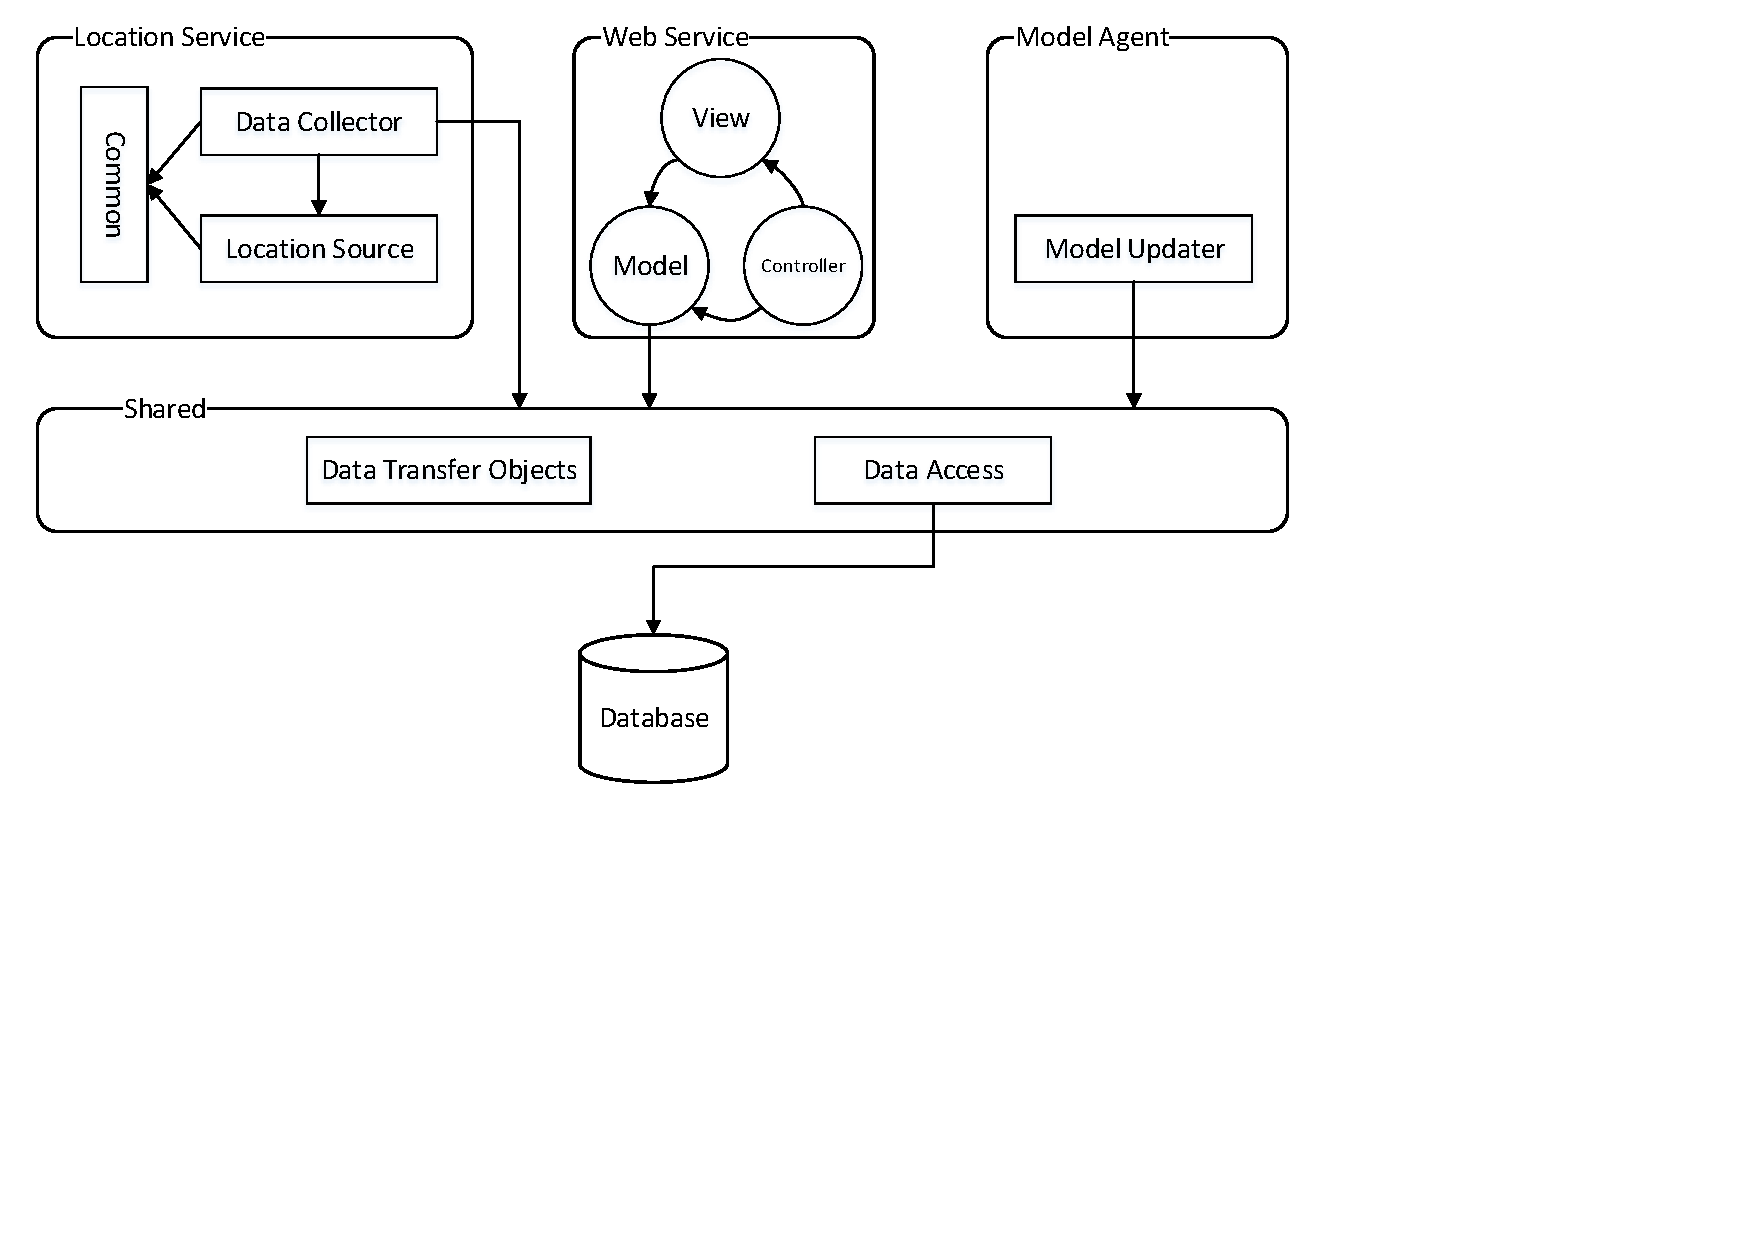
\includegraphics[width=\textwidth, trim={0 8.5cm 8cm 0}]{systemArchitecture.pdf}
\caption{The architecture of the system}
\label{fig:architecture}
\end{figure}

\subsection*{Database} The database used is a MySQL database, and is where all our data is stored.
The design of the database can be found in \cref{database_design}


\subsection*{Shared}\texttt{Shared} is the macro component containing the \texttt{Data Access} layer and the \texttt{Data Transfer Object} layer.
The macro component's task is to provide extended capabilities to all other macro components.

\paragraph{The Data Access layer} All SQL statements and communication with the database are encapsulated here providing the upper layers methods to communicate with the database.

\paragraph{The Data Transfer Object layer} contains all the shared data types and their attributes, making it possible for all the macro components to treat the data uniformly.

\subsection*{Location Service} processes and stores location data directly from a data source. 
The \texttt{Location Service} consists of a \texttt{Location Source} which provides data points the \texttt{Data Collector}.

\paragraph{The Location Source layer} fetched data from the data source then adapts and casts the data to the appropriate data type in the \texttt{Common} layer.
It is structured so the \texttt{Location Source} layer can easily be replaced with another source of data.

\paragraph{The Data Collector layer} gathers the data from the \texttt{Location Source} layer and processes it. 
The data is then stored through the \texttt{Data Access} layer.


\subsection*{Model Agent\footnote{An agent is defined as a program that invoke a given task, when a condition is satisfied, then returning to a sleeping state, until the condition is satisfied again.\cite{definitionagent}}}\texttt{Model Agent} is the macro component containing the \texttt{Model Updater} layer.
The macro component's task is to generate and update the model in the system. 

\paragraph{The Model Updater layer} handles the calculation and generation of the models.
The generation of the model works as follows:
Clusters are created based on the GPS data in the database
The convex hull of the clusters is calculated and saved as the hotspots of the model.
Markov chains are now created with these clusters as states.

\subsection*{Web Service}\texttt{Web Service} is the macro component containing the \texttt{Model}, \texttt{View}, and \texttt{Controller}.
The task of the macro component is to provide a web service for users to interact with the system.

\paragraph{The Model} manages the application domain and handles data and actions possible for each data type.

\paragraph{The View} manages the display of the \texttt{Model}.

\paragraph{The Controller} handles the user interaction. Based on the user request, the \texttt{Controller} sends commands to the \texttt{Model} and \texttt{View}.